\section{ODEs from reaction rates}
Chemical reactions form a broad field of applications where deterministic and stochastic methads are very useful. Such reactions include a wide class of systems where individuals of some entity encounter rondomly and then react with some others of the same or different entity (reactants) and produce individuals which may be of a different nature (products) w.r.t. the reactants. The systems that can be studied in this fromewark include:

\begin{enumerate}
  \item Actual chamical reactions which invalve particles on molecules which transform upon callisions.
  \item Population systems, where individuals may die, give binth, note, consume each other, immigrate....
  \item Epidemics, where discoses are transmitted from ind. to ind. (infected \& susceptibles)
  \item Gene expression, where genes con be trouscripted (into manA) and trouslated (into proteins) upon the appropriate occurrence of some transcription factors.
  \item ...
\end{enumerate}

These reactions may be reversible on not, according to whether the direct reaction con also occur in the bacteword direction.

In this part of the module we will be only concerned with the deterministic properties of these zystems (meon-field approx.), namely, we will not study their stochastic properties.

We will wite down the DDEs for the concentrations of the reactants and products starting from the consesponding mles that govern the chemical reactions.

Bimory and irrevensible reaction. A molecule of type $x$ and a molec. of type $Y$ (reactants) callide and react to produce a molecule of type $z$ (product):\
(1)

$$
 x+y \xrightarrow{k} z
$$

$K$ is the timetic constant which is used to compute $r(x, y)$, which gives the rote of occurrence of the reaction

$$ 
 2 \mathrm{H}_{2}+\mathrm{O}_{2} \xrightarrow{\mathrm{~K}} 2 \mathrm{H}_{2} \mathrm{O} 
$$ 

stoichiometric coefficients: # of react. or prod. of each type that are consumed or produced in the reaction.

Calculation of the raction wate\
We assume that the reaction occurs in a finite valume $V$ where the molecules are well-stived and the concentrations of $X, Y$ and $Z$ are "small", despite the number of molacules of each type is "larga". We will assume that the concentrations $x=\frac{n_{x}}{v}, y=\frac{n_{y}}{v}, z=\frac{n_{z}}{v}$ ( $n_{i}$ : # of molec. of type $i$ ) are continuous variables. We want to estimate $r(x, y)$, the reaction rate, in the diluted limit cose:\
(2)

$$ 
r(x, y) \simeq r(0,0)+\left(\partial_{x} r_{0}\right) x+\left(\partial_{y} r_{0}\right) y+\left(\frac{1}{2} \partial_{x x}^{2} r_{0}\right) x^{2}+\left(\partial_{x y}^{2} r_{0}\right) x y+\left(\frac{1}{2} \partial_{y y}^{2} r_{0}\right) y^{2}+h_{0} t 
$$ 

suall concentrotions $x, y$\
We expect that $r(0, y)=0$ for all $y$ as well as $r(x, 0)=0$ for all $x$, because we need both $x$ and $y$ for the reaction to occur. Therefore from ef. (2) we get\
$r(0, y)=r(0,0)+\left(\partial_{y} r_{0}\right) y+\left(\frac{1}{2} \partial_{y y}^{2} r_{0}\right) y^{2} \equiv 0 \quad \Rightarrow r(0,0)=0, \partial_{y} r_{0}=0, \partial_{y y}^{2} r_{0}=0$\
$r(0, x)=\partial_{x} r_{0} x+\frac{1}{2} \partial_{x t}^{2} r_{0} x^{2} \equiv 0 \Rightarrow \partial_{x} r_{0}=0, \partial_{x x}^{2} r_{0}=0$\
Hence we are left with

$$ 
 \text { (3) } \quad r(x, y)=\partial_{x y}^{2} r_{0} x y \equiv k x y 
$$ 

Obs: particles are pree to mave and vandomly meet with each other: the prob. of $x$ and $y$ to collide are indip. When they meet, they can react.\
where the kinetic constant $k$ does not depend on concentrotions. $k$ may depend on the temperature, $k=k_{0} e^{-\frac{E}{k T}}$ (Eactivation energy), with the Arrhenius factor $e^{-E / k T}$.

The previans motivetion leads to an approximate/empinical "law" which is simple and useful in mony situations:

\section*{The law of Mass Action}
In a first approximation, the rate of any chemical reaction is proportional to the product of the concentrations of the reacting substances.

We can use this law to deduce the $O D E s$ for the evolution of the concentrations. If we know the concent. at time $t$, then at time $t_{+} \Delta t$ (see q.(1)):
(4)

$$ 
 \begin{aligned}
& x(t+\Delta t)=x(t)-k x(t) y(t) \Delta t \\
& y(t+\Delta t)=x(t)-k x(t) y(t) \Delta t \\
& z(t+\Delta t)=z(t)+k x(t) y(t) \Delta t
\end{aligned} \quad \xrightarrow{\Delta t}\left\{\begin{array}{l}
\dot{x}=-k x y, x(0)=x_{0} \\
\dot{y}=-k x y, y(0)=y_{0} \\
\dot{z}=k x y, z(0)=z_{0}
\end{array}\right.
$$ 

Eq. (4) has a consenvation law:\
$\dot{x}-\dot{y}=0 \quad \Rightarrow \quad x(t)-y(t)=x_{0}-y_{0}=c$ constant Therefore we can simplify ef. (4):\
\begin{center}
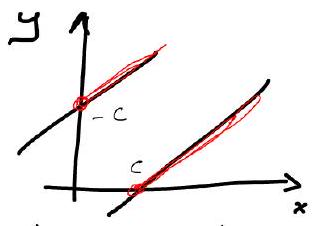
\includegraphics[width=\textwidth]{2025_10_17_109d3ce1ba98c27731a1g-3}
\end{center}


\begin{equation*}
\dot{x}=-k x(x-c)=k x(c-x) \tag{5}
\end{equation*}


This is called lagistic equation and can be solved andytically:\
(6)

$$ 
x(t)=\frac{c x_{0} e^{c k t}}{c+x_{0}\left(e^{c k t}-1\right)} 
$$ 

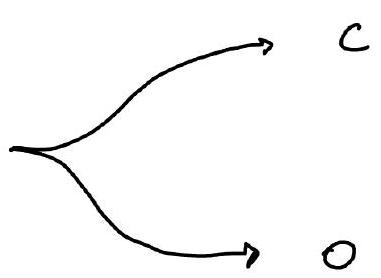
\includegraphics[width=0.5\textwidth]{2025_10_17_109d3ce1ba98c27731a1g-3(1)} if $c>0$ as $t \rightarrow+\infty$
\if $c<0$

Check of (6) out. What happens if $c=0$ ? Solve op. (4) $f_{2} z(t)$. There is another independent consensation law: $\dot{x}+\dot{z}=0 \Rightarrow x(t)+z(t)=x_{0}+z_{0}$ Therefore if $c>0, z \longrightarrow x_{0}+z_{0}-c=z_{0}+y_{0}$ as $t \rightarrow \infty_{j}$ all $y$ goes to $z$. If $c<0, z \rightarrow z_{0}+x_{0}$.\
\begin{center}
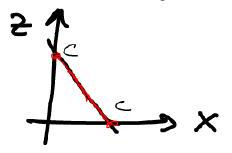
\includegraphics[width=\textwidth]{2025_10_17_109d3ce1ba98c27731a1g-3(2)}
\end{center}

\section*{Binary reversible reaction:}
(7) $x+y \underset{k_{-}}{\stackrel{k_{+}}{\rightleftarrows}} z \quad k_{ \pm}>0$

Along the some lines as before we deduce the evolution of concent. \
(8)

$$ 
 \left\{ \begin{array}{l}
\dot{x}=k-z-k+x y \\
\dot{y}=k \text {, but als decreases because it} \\
\dot{z}=-k-z+k+x y \quad \text { reacts with } r \text { to produce } z) 
\end{array}\right. 
$$ 

Verify that there are two independent conservation laws $x(t)-y(t)=c$, and $x(t)+z(t)=c_{2}$. Hence the $g$. for $x$ con be written as
\n(9)

$$ 
\dot{x}=k_{+} x\left(c_{1}-x\right)+k_{-}\left(c_{2}-x\right) 
$$ 

Obs: even this of. con be solved andytically.

A more complicated cose: the Haber procen. This process was developed by F. Haber in the corly 'goos for producing ammonia on an industrial scale: $N_{2}($ nitrogen $)+3 H_{2}($ hydrogen $) \longrightarrow 2 N_{3}$ (ammonia) We consider then the reaction:\
(10) $X+3 Y \underset{k_{-}}{\stackrel{k_{+}}{\rightleftarrows}} 2 z$

The ODEs for the concentrations are Hen:

\[ 
 \text { (11) } \quad\left\{\begin{array}{l}
\dot{x}=-k_{+} x y^{3}+k_{-} z^{2} \quad \tag{a)}\\
\dot{y}=-3 k_{+} x y^{3}+3 k_{-} z^{2} \\
\dot{z}=-2 k_{-} z^{2}+2 k_{+} x y^{3}
\end{array}\right.
\] 

The otichiometric coefficients enter the ODEs:\
Let's interpret the term $-3 k_{+} x y^{3}$ in ep. (11b)

Eq. (1011) tells us that 3 molecules (or moles) of $Y$ have to collide independently along with one molecule (or mole) of $X$ for the reaction to occur in the forwerd ( + ) direction. Also, becouse for every molecule of $X$, three molecules of $Y$ react, for a decrease in concentration of $x$, there is a three fold decrease in concentration of $Y$. Thus, the storichionstric coefficients affect the pob. of a reaction to occur as well as the relative speed of the reaction. Indeed, $3 \dot{x}=\dot{y}$, which relates the two speeds of reaction.\
The term $3 k-z^{2}$ has a similar interpretation: for producing $Y$, two molecules (moles) of $Z$ have to colliole which will generate 3 molec. of $Y$. Also, for every 2 molec. of $z$ that decampose in the backward direction ( $k_{-}$), there will be 3 molec. of $Y$. This means that the speeds of reaction are $3|\dot{z}|=2|\dot{y}|$. If we look at ep. 11.b,c we get $3 \dot{z}=-2 \dot{y}$ becouse the decrease of $Y$ leads to an imcrease of $z$ and vice versa.

Obs: at stationarity $\frac{x y^{3}}{z^{2}}=\frac{k_{-}}{k_{+}}$, but there are also some conservation lows:

$$ 
 3 x(t)-y(t)=c_{1}, \quad 2 x(t)+z(t)=c_{2}, \quad 2 y(t)+3 z(t)=c_{3} 
$$ 

Can you see why these quantities are conserved and why $c_{7}, c_{2}$ and $c_{3}$ are not independent?

More generally, we can restate the law of mass action as

\section*{The law of Mass Action}
In a first approximation, the rate of any chemical reaction is proportional to the product of the concentration of the reacting substonces, where every concentrotion is raised to a power equal to the corresponding stoichiometric coefficient which also has to be included in the reaction speed with the appropriate sign.

Ex: write down the rote equation for the veressible reaction in $9 \cdot(1)$

$$ 
 2 \mathrm{H}_{2}+\mathrm{O}_{2} \underset{k_{-}}{\stackrel{k_{t}}{\rightleftarrows}} 2 \mathrm{H}_{2} \mathrm{O} 
$$ 

The general veaction\
(12) $a X+b Y \underset{k_{-}}{\stackrel{k_{+}}{\rightleftarrows}} c z+d W \quad a, b, c, d \in \mathbb{N}$

leads to the following odes:

$$ 
 \left\{\begin{array}{l}
\dot{x}=a\left(-k_{+} x^{a} y^{b}+k_{-} z^{c} w^{d}\right) \\
\dot{y}=b\left(-k_{+} x^{a} y^{b}+k_{-} z^{c} w^{d}\right)
\dot{z}=c\left(+k_{+} x^{a} y^{b}-k_{-} z^{c} w^{d}\right) \\
\dot{w}=d\left(+k_{+} x^{a} y^{b}-k_{-} z^{c} w^{d}\right)
\end{array}\right. 
$$ 

Calculate the quontities that are conserved.\
There are types of molecules or species that can interact in different kinds of reactions:\
The predator $(Y)$ and prey $(X)$ system: (isseversible reactions)


\begin{align*}
 X & \xrightarrow{k_{1}} 2 X \\
 Y+X & \xrightarrow{k_{2}} 2 Y \quad \tag{13}\\
 Y & \xrightarrow{k_{3}} \phi
\end{align*} 

reproduction of preys predator eats a prey predator dies.

To get the DDES we have simply to sum the effects of different reactions:\
(14) $\quad\left\{\begin{array}{l}\\dot{x}=k_{1} x-k_{2} x y \\
\\dot{y}=k_{2} x y-k_{3} y
\end{array}\right.$

These are the Lotka-Volterre equations. Show that at stationarity $\bar{x}=\frac{k_{3}}{k_{2}}, \bar{y}=\frac{k_{1}}{k_{2}}$ but the Jacobion at $(\bar{x}, \bar{y})$ has eigenvalues $\lambda= \pm i \sqrt{k_{1} k_{3}}$. as the system stable? Show that $V(x, y)=k_{2}(x+y)-k_{3} \ln x-k_{1} \ln y$ is a conserved quantity.

\section*{General chemical reactions}
More generally we may consider $m$ different chemical species $x_{i}, i=1, 2 \ldots m$ which are invalved in $n$ different reactions of the form
\n(15) $\sum_{\substack{i=1 \ \text { different peries }}}^{m} a_{i j} X_{i} \underset{\substack{\text { different } \ \text { vection }}}{\stackrel{k_{j}^{+}}{\rightleftarrows}} \sum_{i=1}^{m} b_{i j} X_{i} \quad j=1, 2, \ldots, n$

where $a_{i j}$ and $b_{i j}$ are otoichiometric coefficients that ore all non-negative integers.

Therefore the $O D E$ s are


\begin{equation*}
\dot{x}_{i}=\sum_{j=1}^{n}\left(b_{i j}-a_{i j}\right) r_{j}(\bar{x}) \quad i=1, 2, \ldots m \tag{16}
\end{equation*} 


where $r_{j}(\bar{x}) \equiv k_{j}^{+} \prod_{i=1}^{m} x_{i}^{a_{i j}}-k_{j}^{-} \prod_{i=1}^{m} x_{i}^{b_{i j}} \quad$ for any $j=1, 2, \ldots, n$.\
We want to find the consensation laws of ep. (16).\
Let $S$ be the stoichiometric matrix: $S_{i j} \equiv b_{i j}-a_{i j}$ This is a $m \times n$ matrix.\
In vector form ep. (16) reads\
(17) $\frac{d}{d t} \vec{x}=S \vec{r}(\bar{x})$

A linear conserv. law for the system (15) or (16) has the frum (if it exists)
\n(18) $\frac{d}{d t} \sum_{i}^{m} c_{i} \cdot x_{i}=0$
\nwhere $c_{i}$ are (not all zero) constants. Of $\sum_{i} c_{i} x_{i}(t)$ is a constant of motion

$$ 
 \sum_{i} c_{i} x_{i}(t)=\sum_{i} c_{i} x_{i}(0)=\vec{c}^{\top} \cdot \vec{x}(0) 
$$ 

where $\vec{c}^{\top}=\left(c_{1}, c_{2}, \ldots, c_{m}\right)$. If we multiply ef (17) by $\vec{c}^{\top}$, then\
(19) $\vec{c}^{\top} \cdot \frac{d}{d t} \vec{x}=\vec{c}^{\top} \cdot s \vec{r}=\frac{d}{d t} \vec{c}^{\top} \cdot \vec{x}(0)=0$

Eq. (19) halds true for all $\vec{r}$, hence it must be

$$ 
 \text { (20) } \quad \vec{c}^{\top} S=0 \quad \text { or } \quad S^{\top} \vec{c}=0 
$$ 

The consenation laws of the system of reactions in ef - (16) ore given by the non-zero elements $\vec{C} \in \operatorname{ker}\left(S^{\top}\right)\left(\vec{C}^{\top} \cdot \vec{x}=\right.$ const $)$ and the mumber of (lineorly independent) consesistion laws is given by $\operatorname{dim}\left(k e r\left(s^{\top}\right)\right)$. For the reaction $x+y \rightarrow z, s=\begin{pmatrix}-1 \ -1 \ 1\end{pmatrix}, \operatorname{ker}\left(\delta^{\top}\right)=\left\{\left(c_{1}, c_{2}, c_{3}\right) \mid c_{1}+c_{2}=c_{3}\right\}, \operatorname{dim}\left[\operatorname{ken}\left(s^{\top}\right)\right]=2 \sum_{i} c_{i} x_{i}=c_{1} x+c_{2} y+\left(c_{1}+c_{2}\right) z=\text { const }. \text { Bosis } (1,-1,0) \text { and } (1,0,1) \rightarrow x-y=\text{ const.} 

$$ 
x+z=\text { const. } 
$$ 

Tools for the simulation of chemical reactions\
Many tools and libroines are availoble for the mumerical simulation of chemical reactions:

\begin{verbatim}
 hHp://copasi.ong/                             COPASI                (free and professional)
 htp:// libroadrunner.og/                      LIBROADRUNNER         (for c++/Python)
 sbml.ag/SBML_Softwore_Guide/SBML_ Softwore_Summary                  (for a list)
\end{verbatim}

It is good proctice to write down your own code for you to check whether you have understoad the basics of the theory.

Also, these reactions should be implemented with stochastic algorithms which account for the discrete noture of the porticles. These tools will be provided in the other port of the module.